\begin{frame}
\frametitle{Breathing}
\begin{columns}[c] % The "c" option specifies centered vertical alignment while the "t" option is used for top vertical alignment

\column{.3\textwidth} % Left column and width
%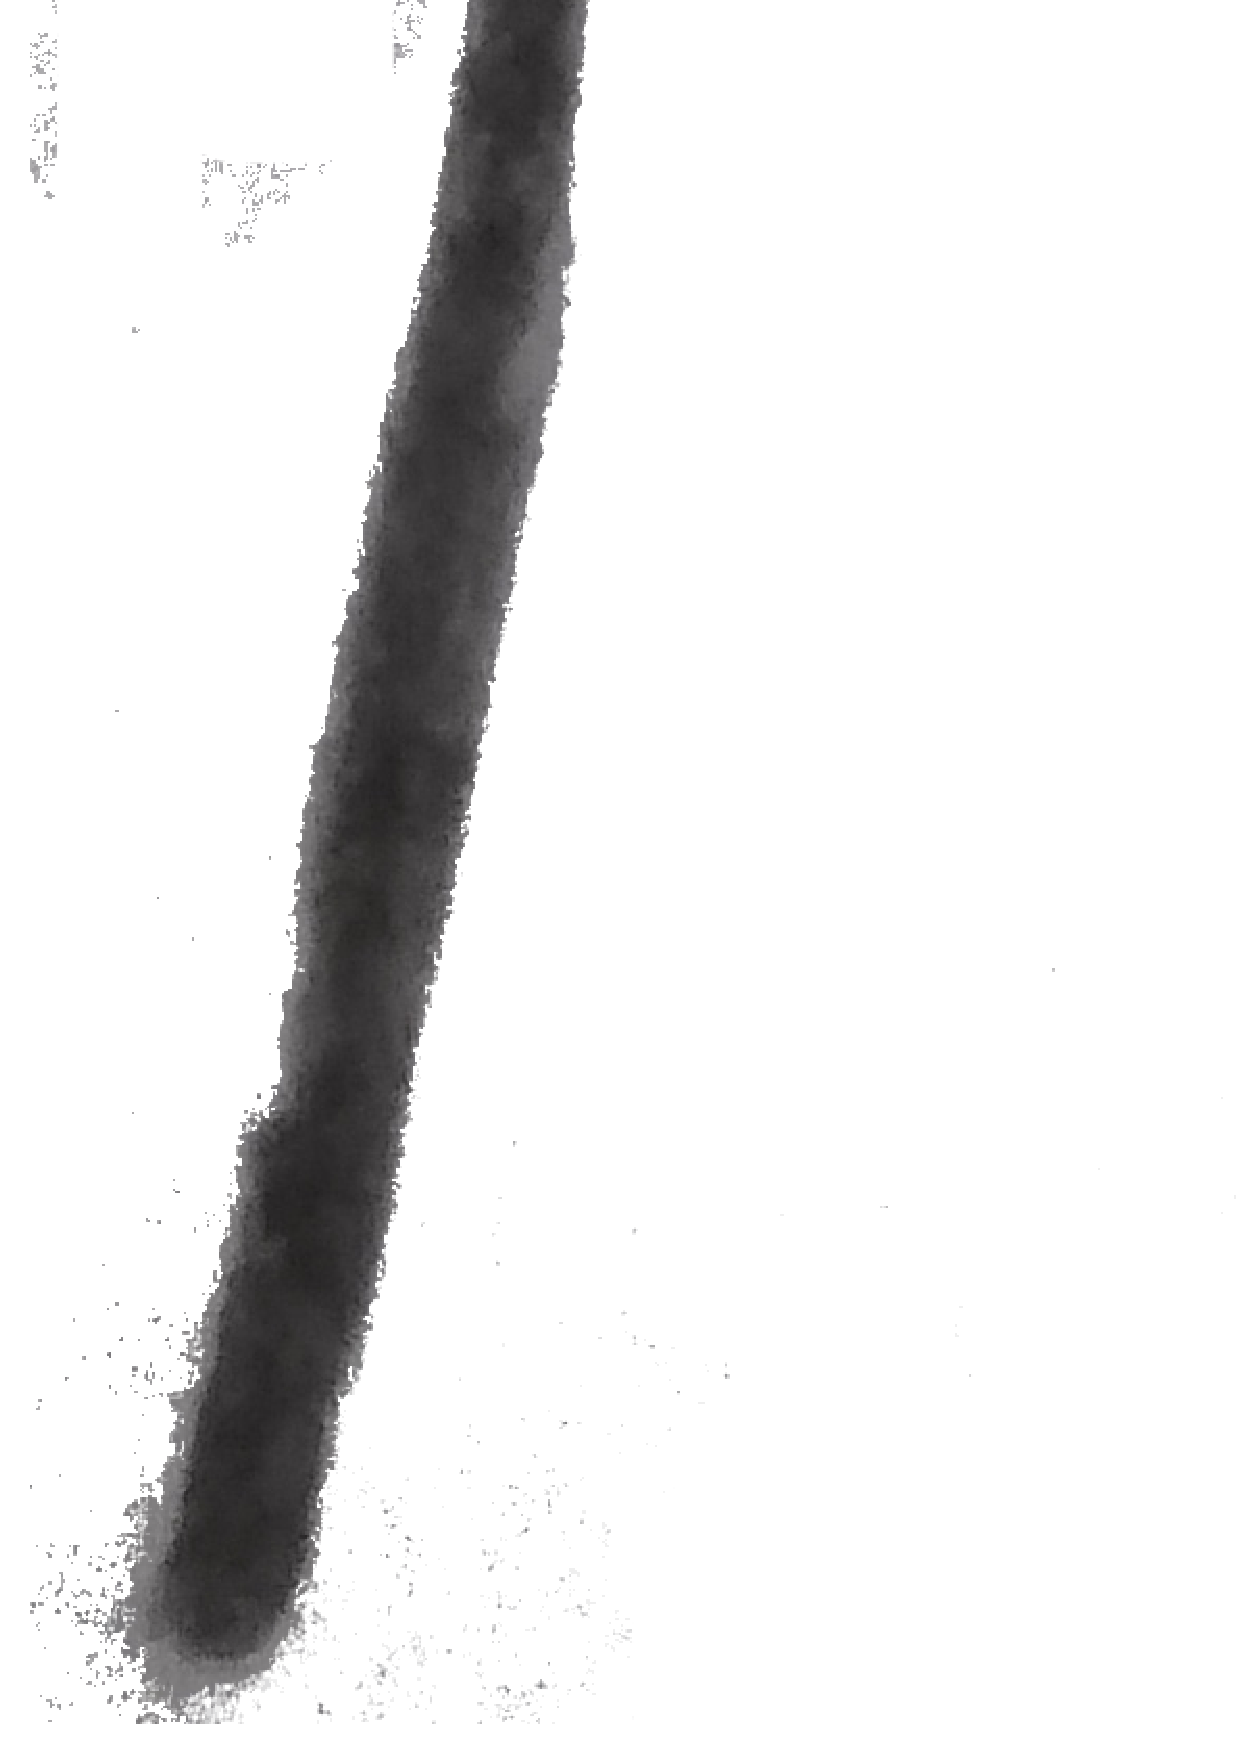
\includegraphics[width=\linewidth]{Sitting_chair_side.png}
\column{.7\textwidth} % Right column and width
\begin{itemize}
\item[-] I \structure{feel the crown}, the highest point of the head, I feel into it.
\item[-] I imagine how the \stucture{breaths stream into my body through that point}, in a relaxed manner.
\item[-] And then I \structure{exhale through my feet}.
\item[-] Then I let the breath flow \structure{into my body through the feet} and \structure{out through the tip of my head}.
\end{itemize}
% Write on
\end{columns}
\end{frame}
%--------------------------------------------------------------------------------------------------------------

\begin{frame}
\frametitle{Breathing}
\begin{columns}[c] % The "c" option specifies centered vertical alignment while the "t" option is used for top vertical alignment

\column{.3\textwidth} % Left column and width
%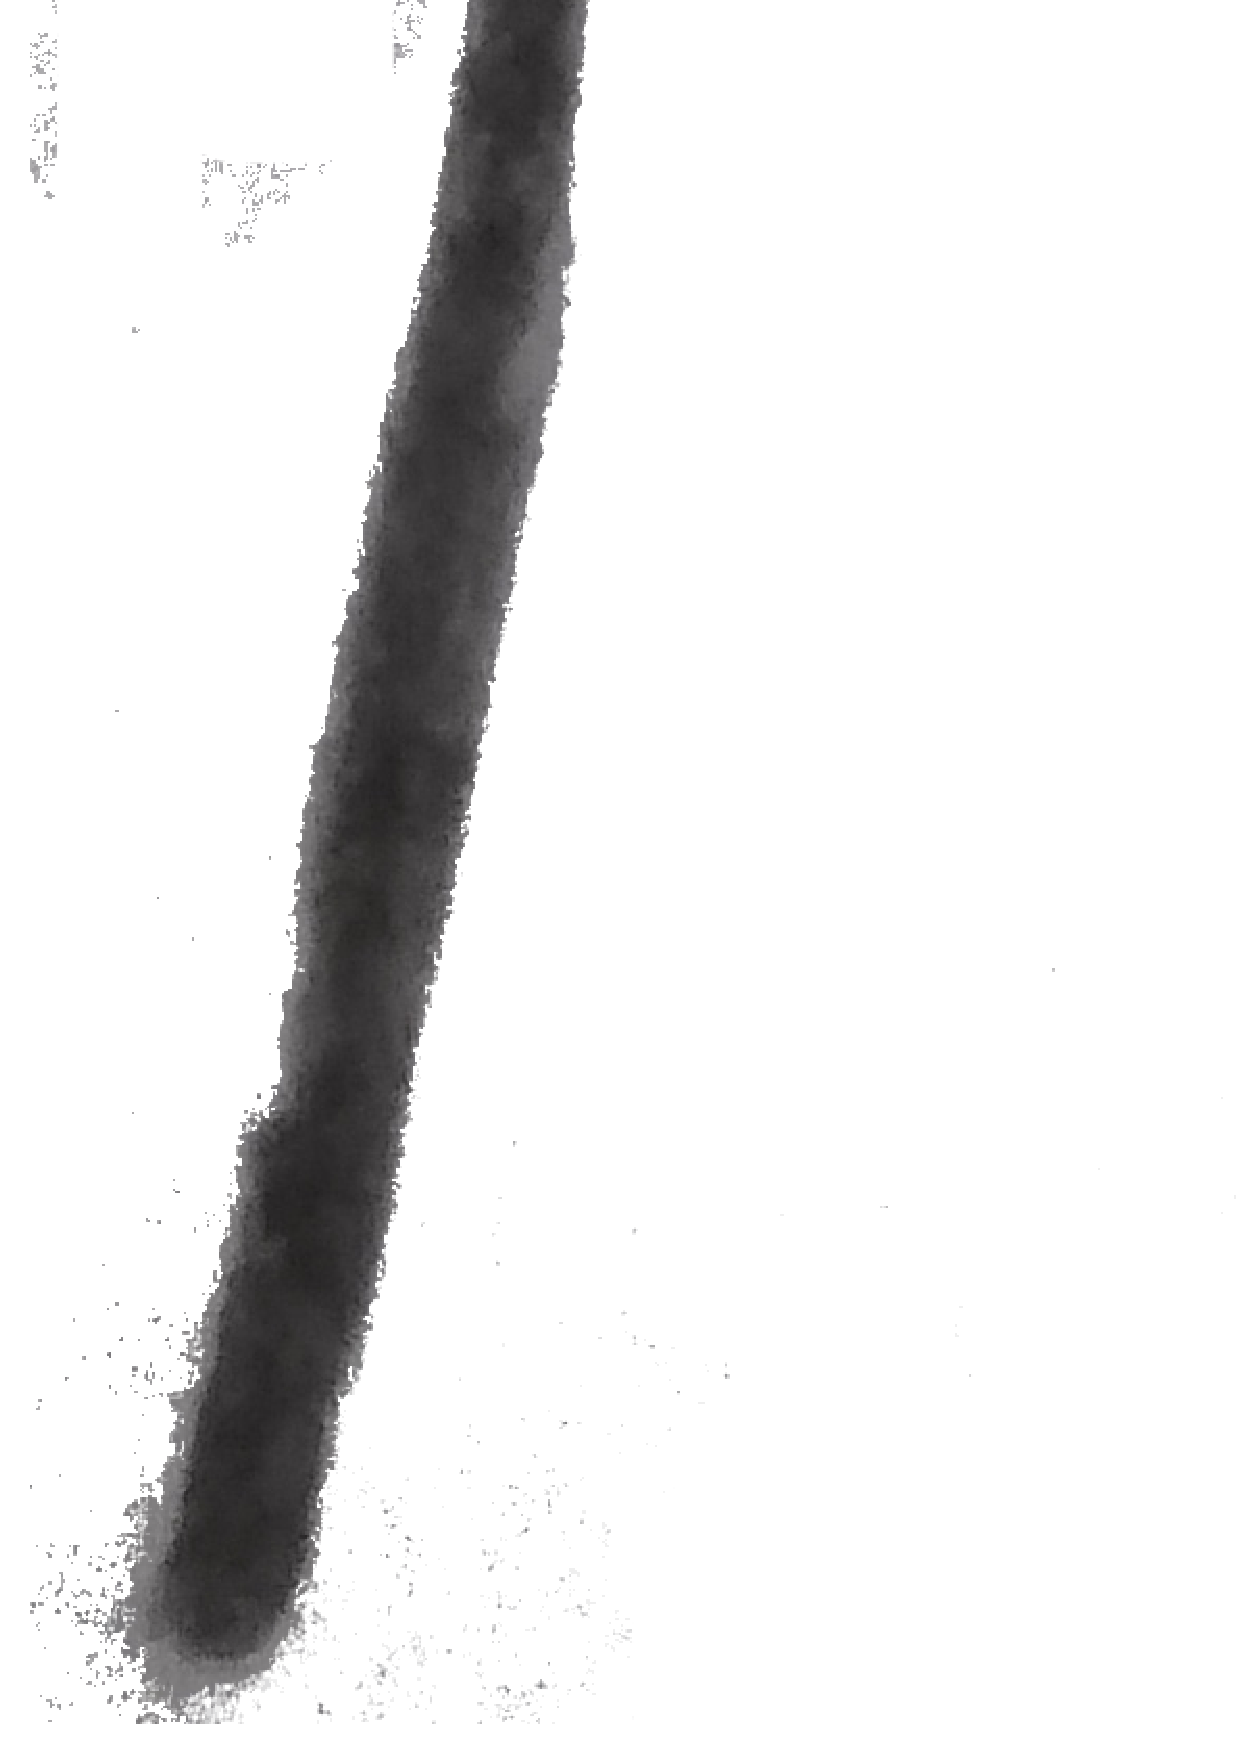
\includegraphics[width=\linewidth]{Sitting_chair_side.png}
\column{.7\textwidth} % Right column and width
\begin{itemize}
\item[-] nnn

  \end{itemize}
% Write on
\end{columns}
\end{frame}
%--------------------------------------------------------------------------------------------------------------
